\documentclass[portrait,final,a0paper,fontscale=0.33]{baposter}

%% read in constants, custom functions and used packages

%%%%%%%%%%%%%%%%%%%%%%%%%%%%%%%%%%%%%%%%%%%%%%%%%%%%%%%%%%%%%%%%%%%%%%%% References paths
\usepackage[backend=biber, style=apa, citestyle=apa]{biblatex}
\addbibresource{refs.bib}
\AtBeginBibliography{\small}

%%%%%%%%%%%%%%%%%%%%%%%%%%%%%%%%%%%%%%%%%%%%%%%%%%%%%%%%%%%%%%%%%%%%%%%% Image paths
\usepackage{graphicx}
\graphicspath{{logos/}{figures/}}

%%%%%%%%%%%%%%%%%%%%%%%%%%%%%%%%%%%%%%%%%%%%%%%%%%%%%%%%%%%%%%%%%%%%%%%% Color Settings
\usepackage{xcolor}
\definecolor{iftucfont}{RGB}{74,130,70}
\definecolor{iftuccolor}{RGB}{143,168,92}
\definecolor{iftucbackground}{RGB}{241,244,234}

%%%%%%%%%%%%%%%%%%%%%%%%%%%%%%%%%%%%%%%%%%%%%%%%%%%%%%%%%%%%%%%%%%%%%%%% Font Settings
\usepackage[sfdefault, regular]{roboto}

%%%%%%%%%%%%%%%%%%%%%%%%%%%%%%%%%%%%%%%%%%%%%%%%%%%%%%%%%%%%%%%%%%%%%%%% Multicol Settings
\usepackage{multirow}
\usepackage{multicol}
\setlength{\columnsep}{1.5em}
\setlength{\columnseprule}{0mm}

%% Row Settings
\usepackage{setspace}% for \onehalfspacing
\usepackage{parskip}

%% Control layout of itemize, enumerate, description
\usepackage{enumitem}

% page borders and header height
\usepackage{geometry}
\geometry{
	left=35pt,
	right=5pt,
	top=10pt
}

\newcommand{\compresslist}{% Define a command to reduce spacing within itemize/enumerate environments, e.g. \begin{itemize}\compresslist
			\setlength{\itemsep}{1pt}
			\setlength{\parskip}{0pt}
			\setlength{\parsep}{0pt}
		}
	
\newcommand{\compressbib}{%
		\setlength{\itemsep}{0pt}
		\setlength{\parskip}{0pt}
		\setlength{\parsep}{0pt}}
	
%%%%%%%%%%%%%%%%%%%%%%%%%%%%%%%%%%%%%%%%%%%%%%%%%%%%%%%%%%%%%%%%%%%%%%%% Table and figure settings
\usepackage{float, booktabs,array}

% Adjust row width in tables 
\renewcommand{\arraystretch}{1.1}

% for awesome plots and tables from files like .csv
\usepackage{pgfplots}
\usepackage{pgfplotstable}

% Graphics package-alike macros for “general” boxes. Like resizing figures and aligning minipages
\usepackage{adjustbox}

\usepackage[
font=footnotesize,
labelfont=bf,
%labelfont=sc, %Kapitälchen, passt nicht wg. nicht-osf Ziffern
%%%%labelfont=it, %italics, 
%%%labelfont=sl, %slanted,
hypcap=true,
format=hang,
%margin={2cm,2cm}
width=0.8\linewidth
]{caption}

%%%%%%%%%%%%%%%%%%%%%%%%%%%%%%%%%%%%%%%%%%%%%%%%%%%%%%%%%%%%%%%%%%%%%%%% Other packages
% to help with long equations
\usepackage{amsmath}

% for todo notes
\usepackage{todonotes} 

% for comment blocks
\usepackage{verbatim}

% link URLs
\usepackage{url}

\usepackage{lipsum}


\begin{document}

\begin{poster}%
	% Poster Options
	{
		% Show grid to help with alignment
		grid=false,
		% Number of columns and column spacing
		columns=6,
		colspacing=1em,
		% Color style
		bgColorOne=white,
		borderColor=iftuccolor,
		headerColorOne=iftucbackground,
		headerFontColor=iftucfont,
		boxColorOne=white,
		% Format of textbox
		textborder=rounded,
		textfont=\small,
		% Format of text header
		eyecatcher=true,
		headerborder=closed,
		headerheight=0.1\textheight,
		%  textfont=\sc, An example of changing the text font
		headershape=rounded,
		headershade=plain,
		headerfont=\Large\bf, %Sans Serif
		% textfont={\setlength{\parindent}{1.5em}},
		boxshade=plain,
		%  background=shade-tb,
		background=plain,
		linewidth=2pt
	}
	% University logo
	{
\includegraphics[height=6.5em]{tuckhseng_color}} 
	% Title
	{\bf\Large{Dynamic and adaptive body schema by learning to predict the sensory consequences of actions}\vspace{1em}}
	% Authors
	{\large Erik~Syniawa\textsuperscript{2}, Valentin~Forch\textsuperscript{1} and Fred~Hamker \\ \vspace{0.5em}
	\small Contact: erik.syniawa@informatik.tu-chemnitz.de
	}
	% Department logo and other logos
	{	
		\begin{minipage}[r]{0.1\textwidth}
			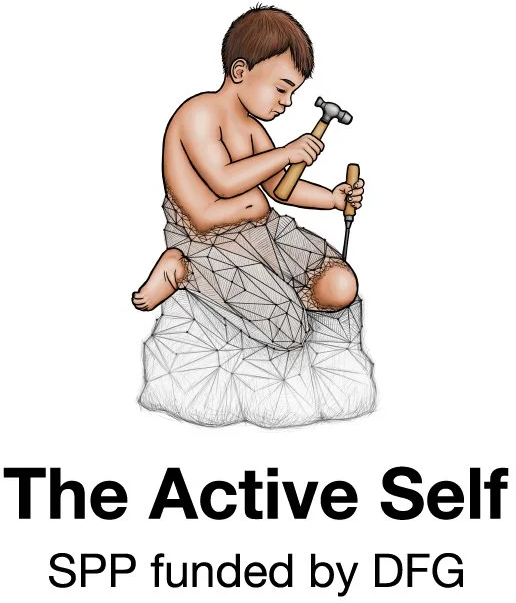
\includegraphics[height=7em]{active_self_logo_color}
		\end{minipage}
		\hfill
		\begin{minipage}[r]{0.1\textwidth}
			
\includegraphics[height=6.5em]{TUC_AI_color}
		\end{minipage}
		
	}

%%%%%%%%%%%%%%%%%%%%%%%%%%%%%%%%%%%%%%%%%%%%%%%%%%%%%%%%%%%%%%%%%%
% use height in headerbox to align multiple boxes 
% height= <size in percent of column height>, else [auto]%
\headerbox{Overview}{name=overview,column=0,row=0, span=4}{
	
	
	\begin{adjustbox}{minipage=0.95\textwidth, margin=5pt, center}
	Systems-level approach to develop a body schema and agency:
	
	\begin{minipage}[l]{0.5\textwidth}
		\begin{itemize}
		\item The \textbf{basal ganglia} will select an action based on the desired state (see \cite{baladronHabitLearningHierarchical2020}).
		\item The \textbf{central pattern generator} will be execute the action (see \cite{nassourConcreteActionRepresentation2020}).
		\item The \textbf{cerebellum} will learn to predict the sensory consequences of the motor action in all modalities (vision, touch, proprioception) i.e. the body schema (see \cite{schmidForwardModelsCerebellum2019}). 
		\item The \textbf{prediction error} will be used to improve the prediction and to train action selection in the \textbf{basal ganglia}.
		\end{itemize}
	\end{minipage}
	\begin{minipage}[r]{0.5\textwidth}
		\raggedleft
		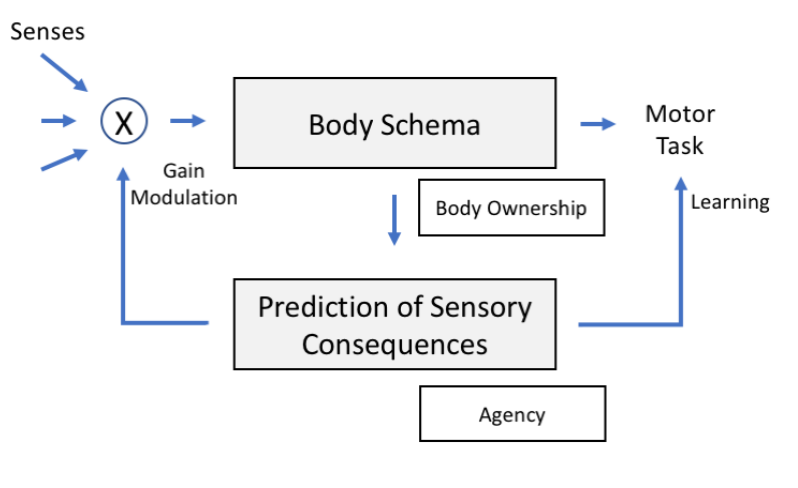
\includegraphics[width=0.9\linewidth]{interplay_bs_motor.png}
		\captionof{figure}{babbas}
	\end{minipage}

	
	\vspace{0.3em}
	\end{adjustbox}
}

\headerbox{\large Sensory Integration\textsuperscript{1}}{name=rbf, column=0, below=overview, span=2, height=0.29}{
	\begin{adjustbox}{minipage=0.95\textwidth, margin=5pt, center}
		\textbf{\small Recurrent Basis Functions (RBF):} \\
		
		RBF have been proposed as a model for multisensory integration and transformation between these frames of reference \parencite{pougetComputationalPerspectiveNeural2002}. \\
		Figure 2 shows an example where the position of the eyes and a joint are used to predict the position of a stimulus in retinocentric coordinates and vice versa.
	
		\vspace{1em}
		\begin{center}
			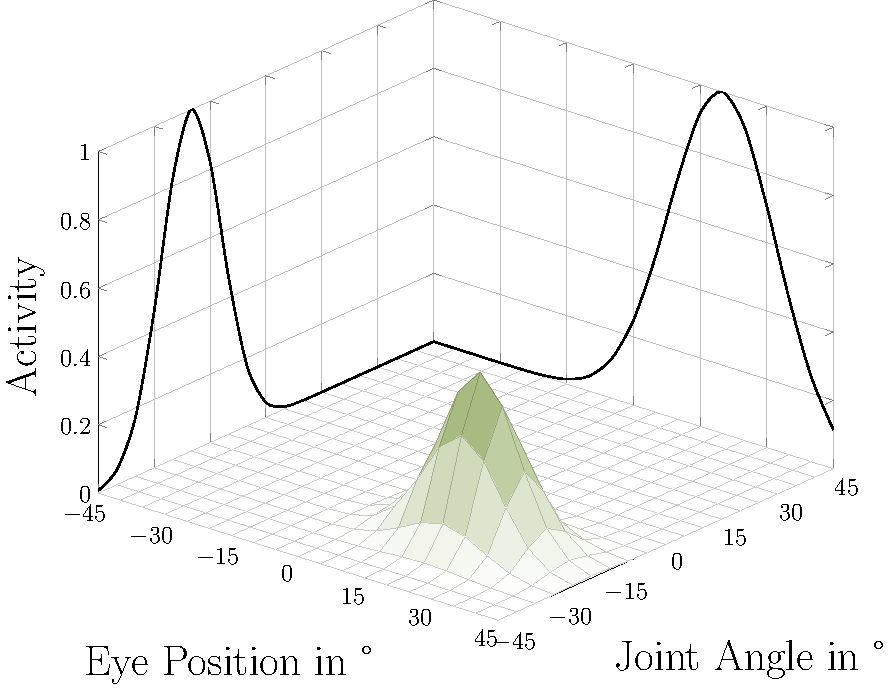
\includegraphics[width=0.8\linewidth]{pop_code_figure}
			\captionof{figure}{Representation of a RBF population code}
		\end{center}
	\end{adjustbox}
}

\headerbox{\large Learning a Body Schema\textsuperscript{1}}{name=network, column=2, below=overview, span=4, height=0.29}{
	\begin{adjustbox}{minipage=0.95\textwidth, margin=5pt, center}
	% Network definitions
	\begin{minipage}[l]{0.30\textwidth}
		\textbf{Rate-coded Neural Network:} \\
		
		Our network simulates neural activity in continuous time and is driven by unsupervised Anti-Hebbian learning \parencite{}. Excitatory neurons learn to represent the statistical features of their inputs while
		inhibitory interneurons decorrelate the excitatory responses leading to a sparse neural code. \\
		
		\textbf{Neuron Model:} \\
		\footnotesize
		$$\tau^{m} \frac{d m_{j} }{d t} + m_{j} = \sum_{j}{w_{ij} \cdot r_{i} } - \sum_{k}{c_{kj} \cdot r_{k} }$$
		 
		$$\tau^{\theta} \frac{d \theta_{j} }{d t} + \epsilon \cdot sign(\theta_{j}) = (r_{j} - r_{Target})$$
		
		$$r_{j} = \left[\alpha \left(\frac{2}{1 + e^{-\beta(m_{j}-\theta_{j})}} -1 \right) \right]^{+}$$

	\end{minipage}
	\hfill
	% Network Architecture
	\begin{minipage}[r]{0.3\textwidth}

		\begin{center}
			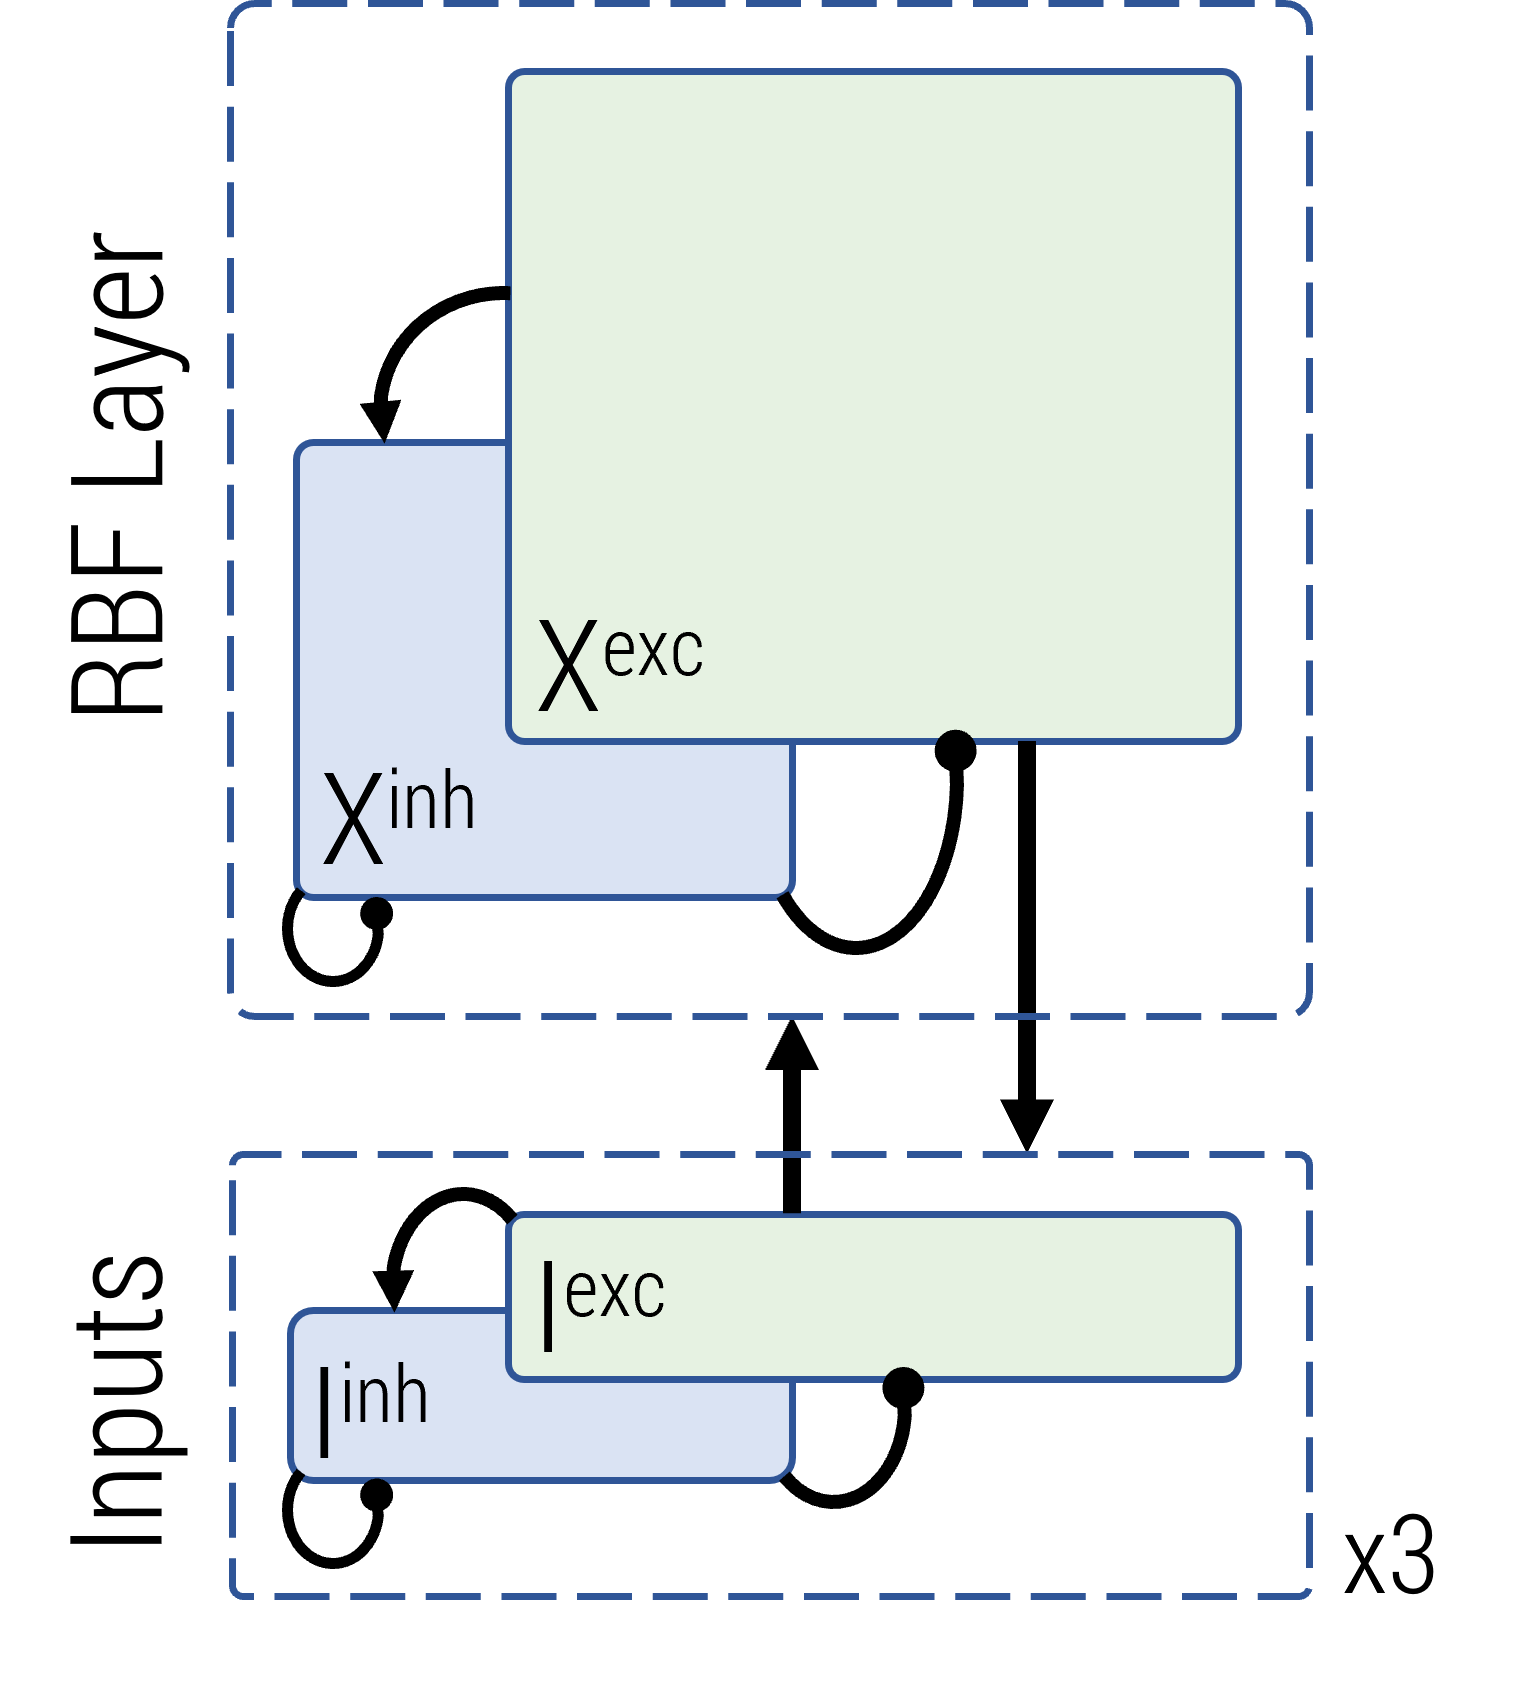
\includegraphics[width=0.8\linewidth]{net}
			\captionof{figure}{Network Architecture}
		\end{center}
		
		\vspace{10pt}
		
		\textbf{Synaptic Learning Rules:} \\
		
		\textit{Excitatory:} 
		\footnotesize
		$$\tau^{ w }\frac{ dw_{ ij } }{ dt } = (r_{ i }-\hat r_{ i }) \cdot r_{j}-\alpha^{w}_{j}r^{2}_{j}w_{ij}$$

		$$\tau^{ \alpha }\frac{ d \alpha^{w}_{j}}{ dt } = \left( \left[ r_{j} - \gamma\right]^{+} \right)^{2} - \alpha^{w}_{j} \text{  with:  }  w_{ij} = \left[w_{ij} \right]^{+}$$
		
		
	\end{minipage}
	\hfill
	% Network Results
	\begin{minipage}[r]{0.33\textwidth}
		\textit{Inhibitory}:
		\footnotesize
		$$\tau^{ c }\frac{ dc_{ kj } }{ dt } = r_{ k } \cdot r_{ j } -\alpha^{c}_{j}r_{j}c_{kj}
		\text{  with:  }  c_{kj} = \left[w_{kj} \right]^{+}$$
		
		\vspace{5pt}
		\small
		\textbf{Results:} \\
		RBF-Neurons develop receptive fields (RF) and show shifting gain
		fields.	This behavior is also found in the cortex \parencite{pougetComputationalPerspectiveNeural2002}.
		
		\vspace{10pt}
		
		\begin{center}
			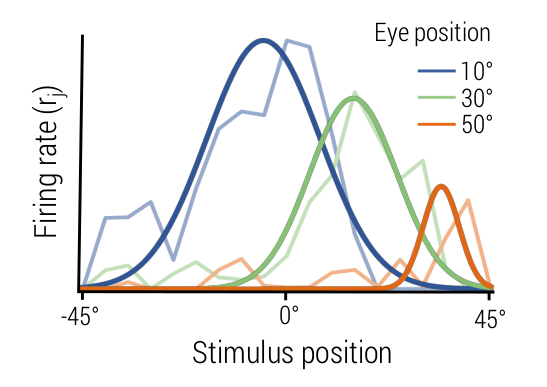
\includegraphics[width=\linewidth]{results_valentin}
			\captionof{figure}{Gain Fields}
		\end{center}

		\hfill
	\end{minipage}

	\end{adjustbox}
}

\headerbox{\large References}{name=refs, column=0, above=bottom, span=6}{
	\begin{adjustbox}{minipage=0.98\textwidth, margin=0pt, center}
		
		\compressbib{\printbibliography[heading=none]}
		
		
	\end{adjustbox}
	
	
}


\headerbox{\large Setup}{name=setup,column=4,row=0, span=2, above=network}{
	\begin{adjustbox}{minipage=0.95\textwidth, margin=5pt, center}
		\vspace{10pt}
		
		\centering
		\includegraphics[width=0.75\linewidth]{robot_setup}
		\captionof{figure}{Current virtual robot setup.}
	\end{adjustbox}
}

\headerbox{\large Basal Ganglia\textsuperscript{2}}{name=bg, column=0, below=rbf, above=refs , span=3}{
	\begin{adjustbox}{minipage=0.95\textwidth, margin=5pt, center}
		
	
		\begin{minipage}[r]{0.48\textwidth}
			\textbf{Network of the Basal Ganglia (BG):}\\
			
			\vspace{2pt}
			\begin{flushright}
				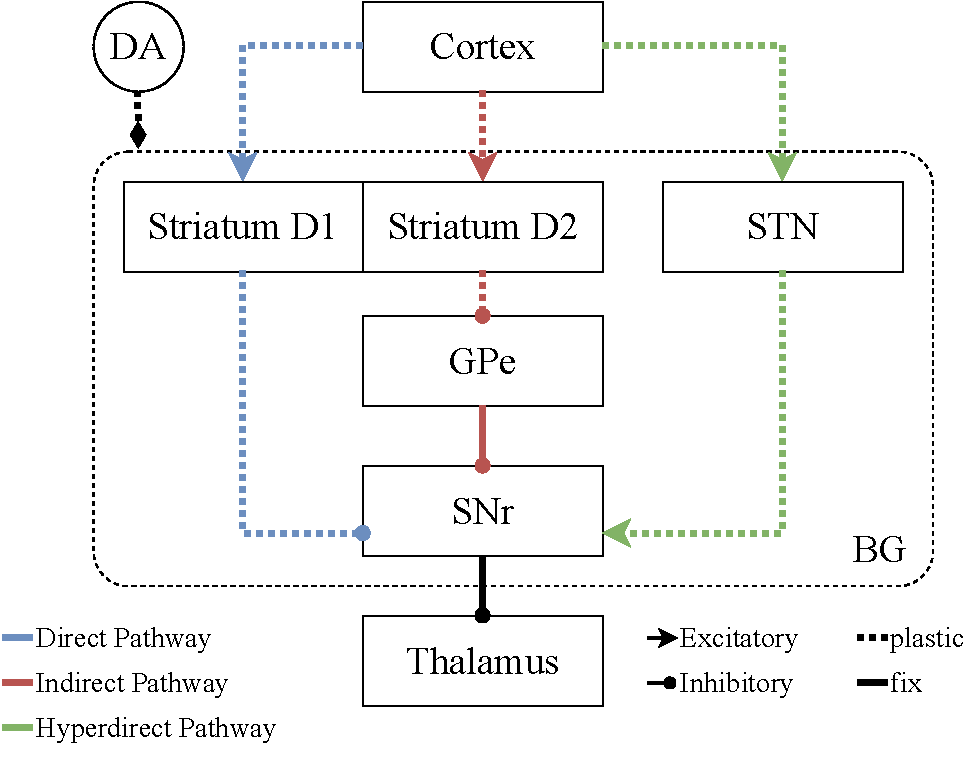
\includegraphics[width=\linewidth]{BG}
				\captionof{figure}{Modeling of segregated \\ basal ganglia pathways}
			\end{flushright}

			
			\vspace{15pt}
			
			Through dopamine-modulated mechanisms, the BG enable motor category learning (Seger, 2008) and are involved in establishing associations between stimulus and responses (Packard \& Knowlton, 2002). Due to the modulating effect of dopamine (DA) on the plasticity of the BG, this model acts as a kind of reinforcement learning agent. \\
			
			
			
			
		\end{minipage}
		\hfill
		\begin{minipage}[l]{0.49\textwidth}
			\textbf{Learning in the different pathways:}\\
			
			The learning principles are primarily determined by presynaptic and postsynaptic activity, as well as the DA-signal (see Table 1). \\
			The labels high and low indicate whether the pre- and post-activity is more than or less than a given threshold (for example, mean population activity).
			DA+ and DA- labels indicate if the SNc activity exceeds a given threshold or not. A sign represents the weight changes in the relevant projections for each combination.
			
			\vspace{10pt}
			
			\resizebox{\columnwidth}{!}{%
	\begin{tabular}{lcccccl}
		\multicolumn{2}{l}{\multirow{4}{*}{}}          & \multicolumn{4}{c}{\textbf{Dopamine}}               & \multirow{4}{*}{}                    \\ \cline{3-6}
		\multicolumn{2}{l}{}                           & \multicolumn{2}{c}{DA +} & \multicolumn{2}{c}{DA -} &                                      \\ \cline{3-6}
		\multicolumn{2}{l}{}                           & \multicolumn{4}{c}{\textbf{Post-activity}}          &                                      \\ \cline{3-6}
		\multicolumn{2}{l}{}                           & High        & Low        & High        & Low        &                                      \\ \hline
		\multirow{12}{*}{\textbf{Pre-activity}} & High & +           &            & -           &            & \multirow{2}{*}{\textbf{Cortex-D1}}  \\
		& Low  & -           &            &             &            &                                      \\ \cline{2-7} 
		& High & -           &            & +           &            & \multirow{2}{*}{\textbf{Cortex-D2}}  \\
		& Low  &             &            & -           &            &                                      \\ \cline{2-7} 
		& High & +           &            & -           &            & \multirow{2}{*}{\textbf{Cortex-STN}} \\
		& Low  & -           &            &             &            &                                      \\ \cline{2-7} 
		& High & -           & +          &             & -          & \multirow{2}{*}{\textbf{D1-SNr}}     \\
		& Low  &             &            &             &            &                                      \\ \cline{2-7} 
		& High &             & -          & -           & +          & \multirow{2}{*}{\textbf{D2-GPe}}     \\
		& Low  &             &            &             &            &                                      \\ \cline{2-7} 
		& High & +           & -          &             & +          & \multirow{2}{*}{\textbf{STN-SNr}}    \\
		& Low  &             &            &             &            &                                      \\ \hline
	\end{tabular}
}
			\captionof{table}{"+"=LTP; "-"=LTD; \\ no sign = no weight change}
		\end{minipage}
	\end{adjustbox}

}

\headerbox{\large Motor Learning with the Basal Ganglia\textsuperscript{2}}{name=motor, column=3, below=network, above=refs , span=3}{

	\begin{adjustbox}{minipage=0.95\textwidth, margin=5pt, center}
		
		\begin{minipage}[l]{0.35\textwidth}
			\textbf{Reaching task:} \\
			
			A goal should be reached in a plane (\textcolor{green}{green}). The BG should choose the right movement trajectory (\textcolor{blue}{blue}) to get from a starting arm position (\textcolor{red}{red}) to arm position to reach the goal (\textbf{black}). See Figure 7.
			
			\vspace{10pt}
			
			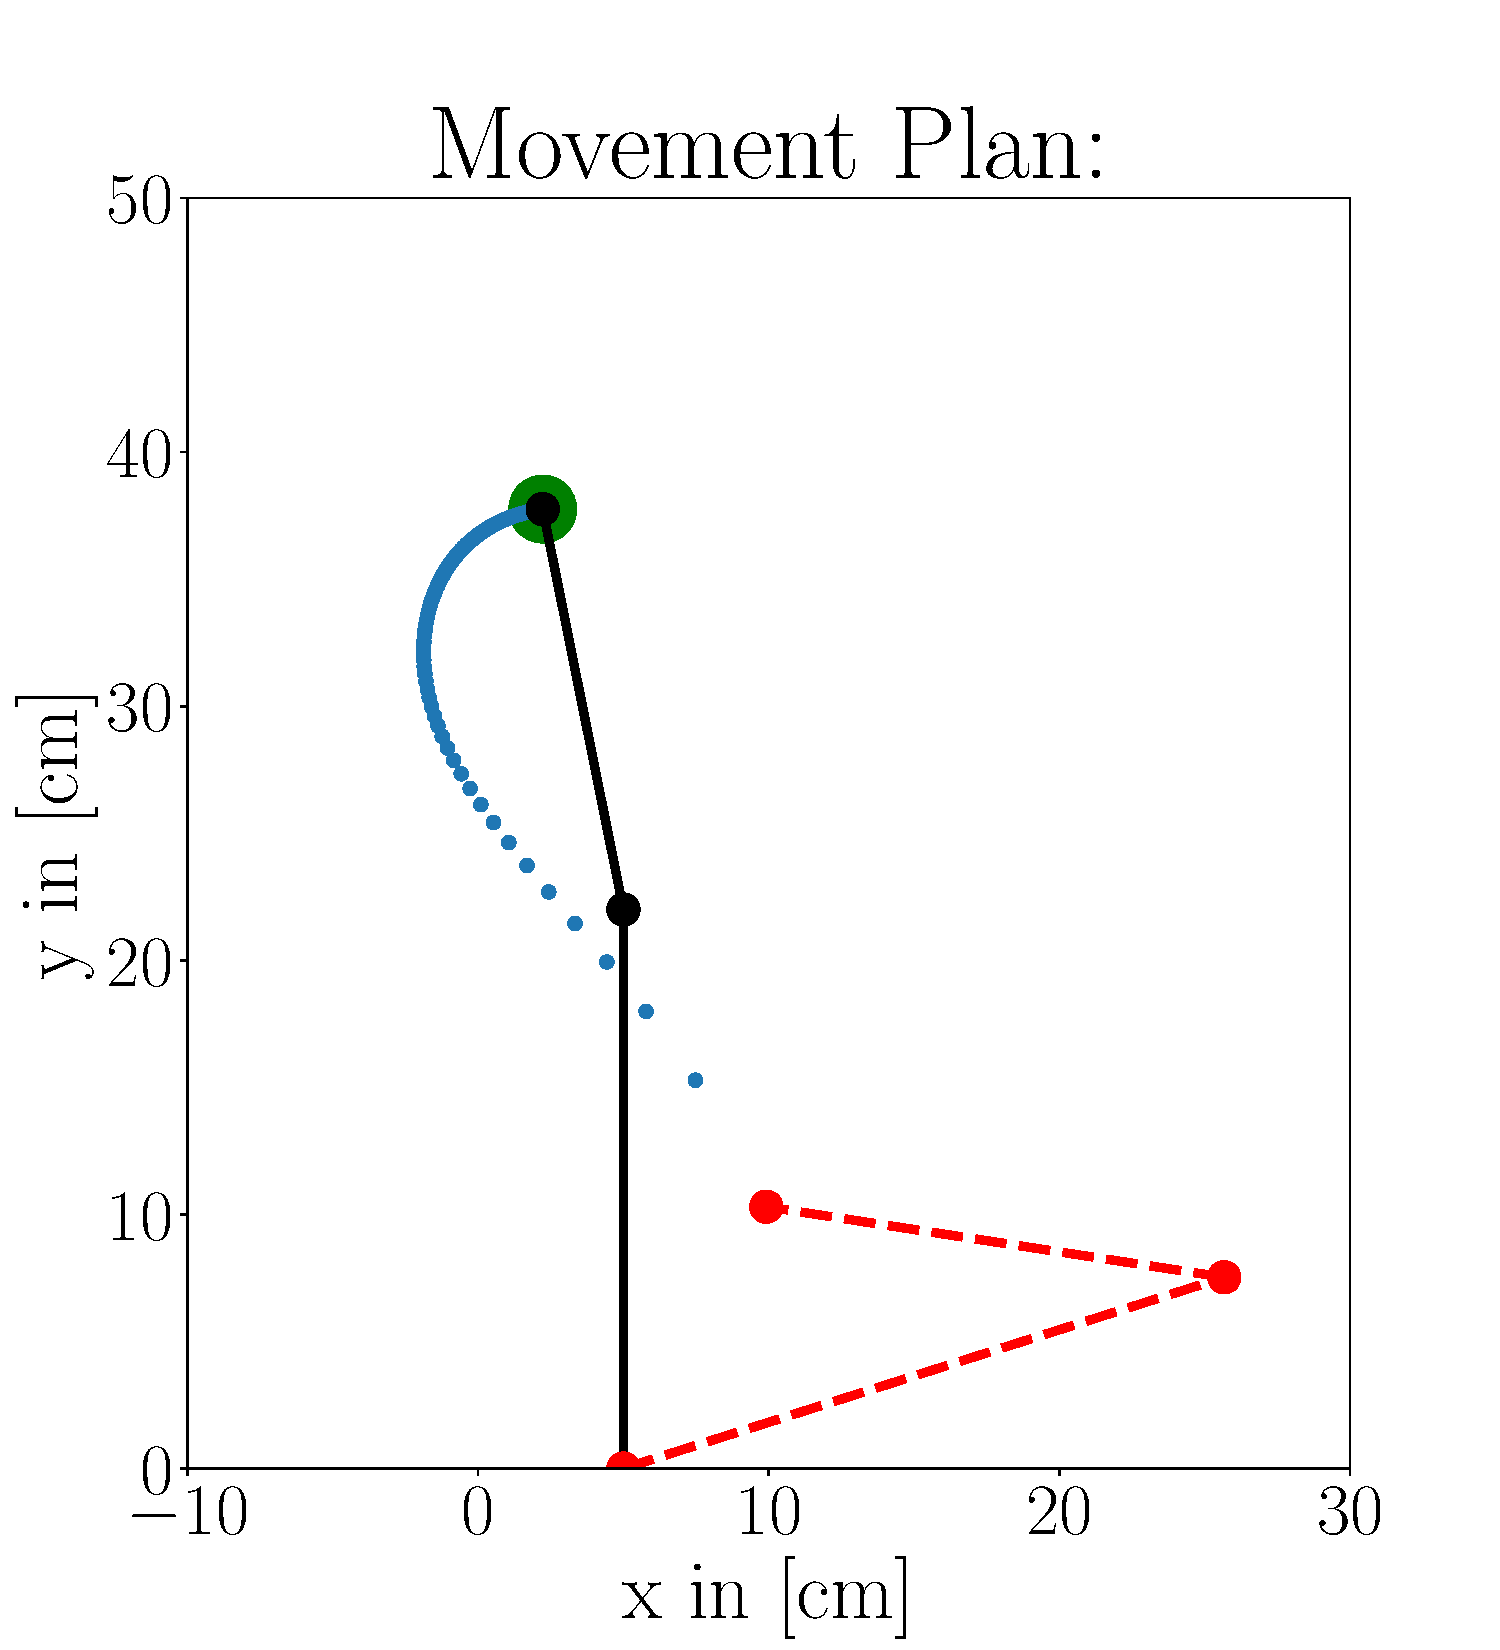
\includegraphics[width=0.9\linewidth]{movement}
			\captionof{figure}{}
			
			\vfill
		\end{minipage}
		\hfill
		\begin{minipage}[r]{0.65\textwidth}
			\vspace{30pt}
			\hspace{6pt}
			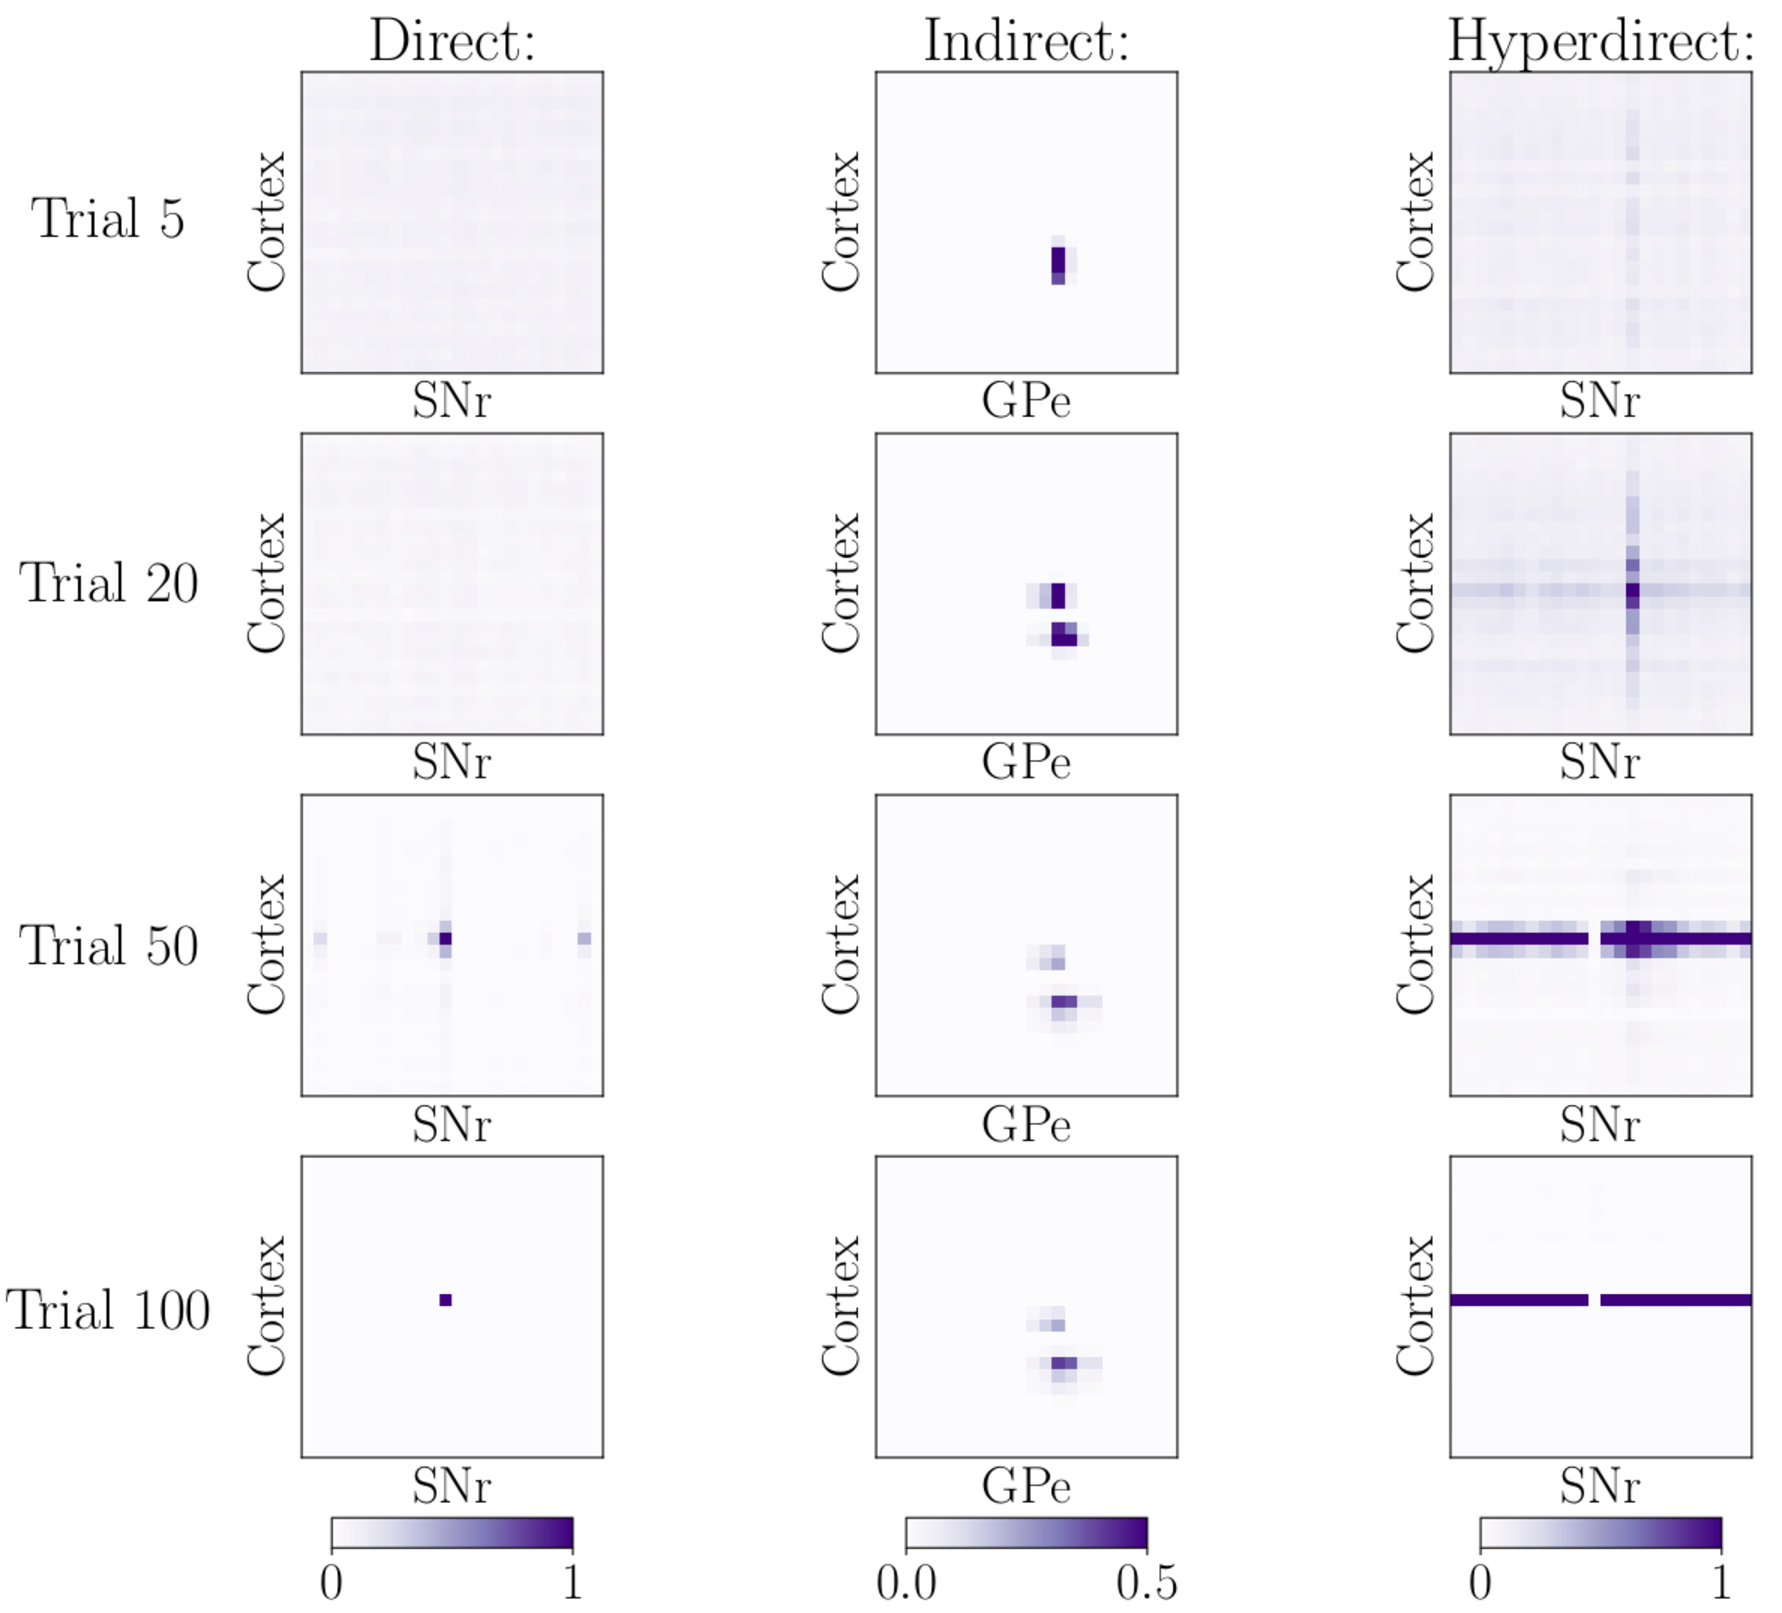
\includegraphics[width=0.98\linewidth]{BG_Learning}
			\captionof{figure}{}
		\end{minipage}
		
		\vspace{5pt}
			
		\begin{minipage}[b]{\textwidth}
			\begin{multicols}{2}
			Figure 8 shows the development of the connection strengths in the different paths.
			At first, unrewarded connections (e.g. movements) are suppressed by the indirect path. Through rewarded selections, a direct and hyperdirect path slowly works its way out. The direct pathway inhibits a neuron associated with rewards in the GPi, while the hyperdirect pathway specifically excites neurons encoding alternative hues in the GPi. This influences the activity of the thalamus so that only one neuron becomes active.
			\end{multicols}
		\end{minipage}
	
	\end{adjustbox}

	

}


\end{poster}


\end{document}